\section{Introduction}
% no \IEEEPARstart
Snake-like robots, with multiple joints and degree of freedom, have strong mobility in complex and unknown terrains\cite{Chirikjian1995The}. Snake-like robots adapt themselves to multiple robotic mobility occasions such as disaster rescuing\cite{DogAndSnake}, factory pipe maintenance\cite{ACMTutorial} and scientific exploration\cite{Kuwada2007Snake}. The early version of snake-like robots used parallel connection structure to connect each two modules, only achieving a plane movement\cite{mori2002three}. Later, with the advent of orthogonal and universal joint structure\cite{1014757}\cite{Date2005Control}\cite{GaitBasedCompliant}, snake-like robots can be applied to three-dimensional space movement, which strengthens snake-like robots' mobility in varied topography. Over the years, more and more gaits that can traverse a variety of terrains, including flat ground and pipes have been developed\cite{5152862}\cite{5602354}. However, it is challenging to make robots move in complex environment without real-time human intervention such as parameters adjustment.

It's necessary for the robots to have autonomous mobility if we want them to move in complex or unknown environment such as climbing the outdoor pipeline for maintenance. Actually, by setting the accurate parameters of motion, snake-like robots can travel along the pipes with different diameters by rolling gait. However, the motions of snake-like robots are not efficient under the real-time control of human. Our goal is to develop a new autonomous control strategy for the motion of snake-like robots. We propose a new control strategy based on learning experience of robots . The robots' adaptive motion can improve adaptability in different movement environments.

This paper applies the new control strategy to the our existing snake-like robot platform, which is shown in \figref{fig:snake_like_robot_a}. The rotation axis of the adjacent joints of our robot are orthogonal and the rotation axis of robot's joints are perpendicular to the its body. We construct the simulation model \figref{fig:snake_like_robot_b} and embed a set of sensors such as accelerometer and gyro to realize the robot feedback control.
\begin{figure}[H]
	\centering
	\subfigure[Reality robot]{
		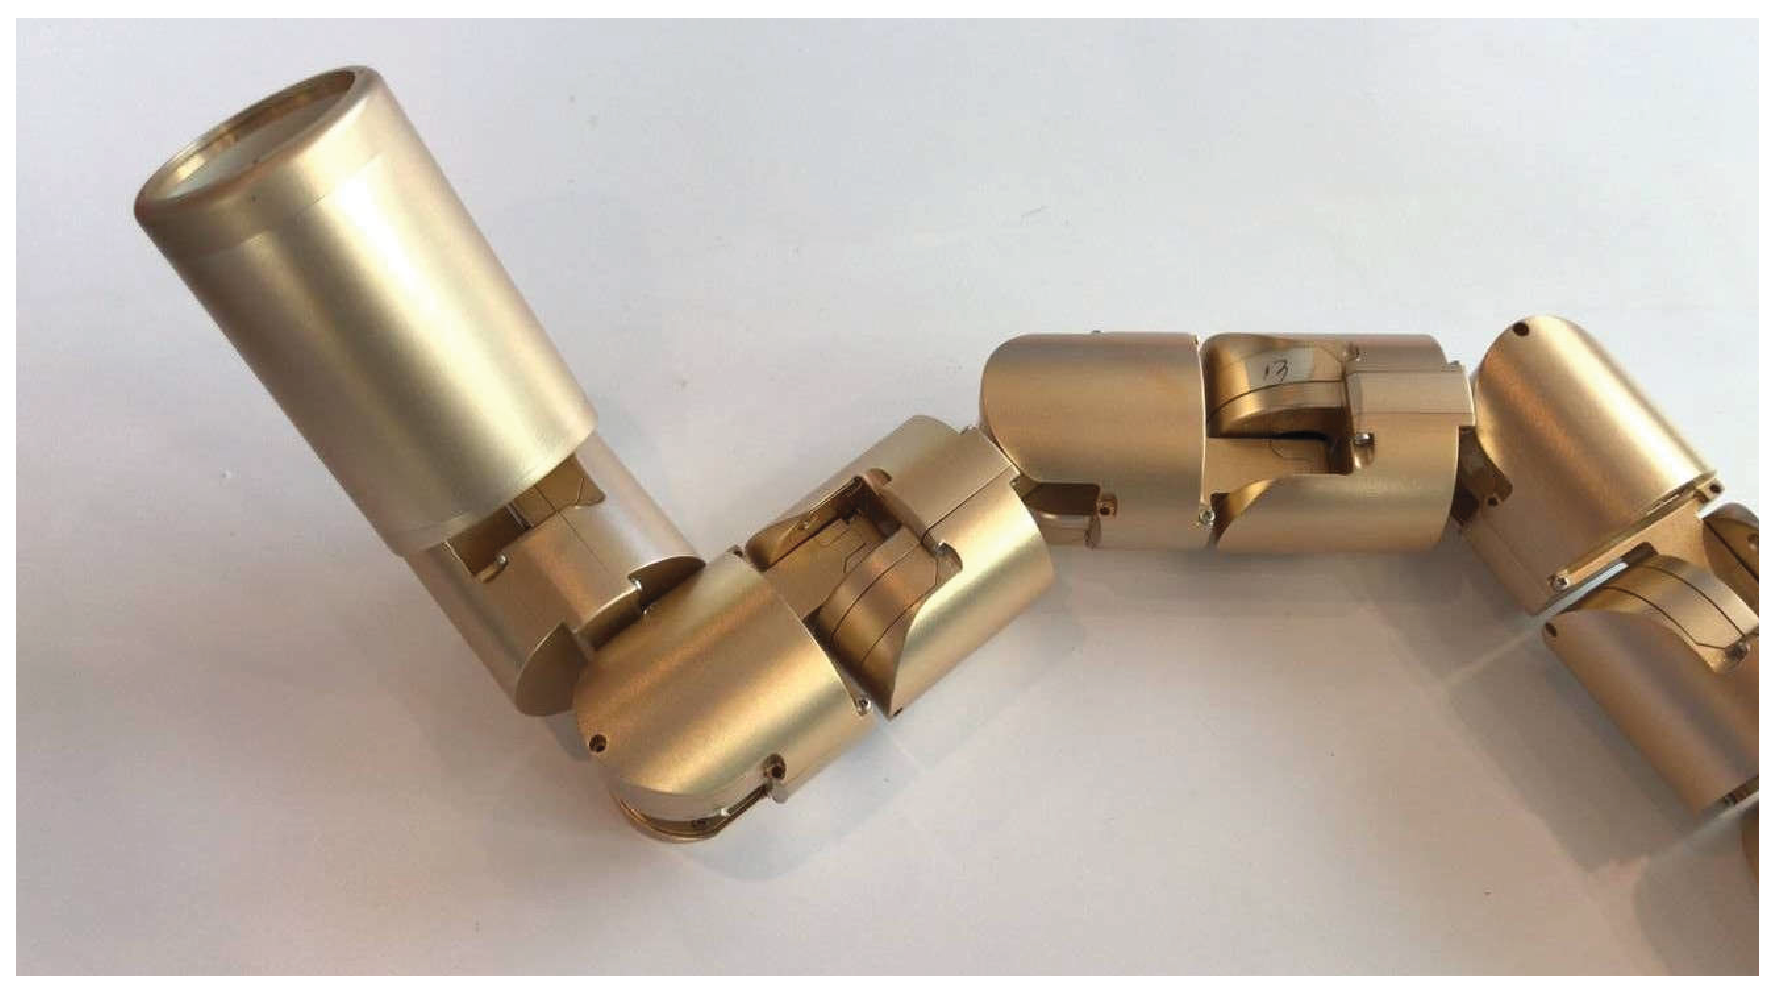
\includegraphics[width=1.5in,height=0.75in]{fig/relative/realSnake}
		\figlabel{fig:snake_like_robot_a}
	}
	\subfigure[Simulate robot]{
		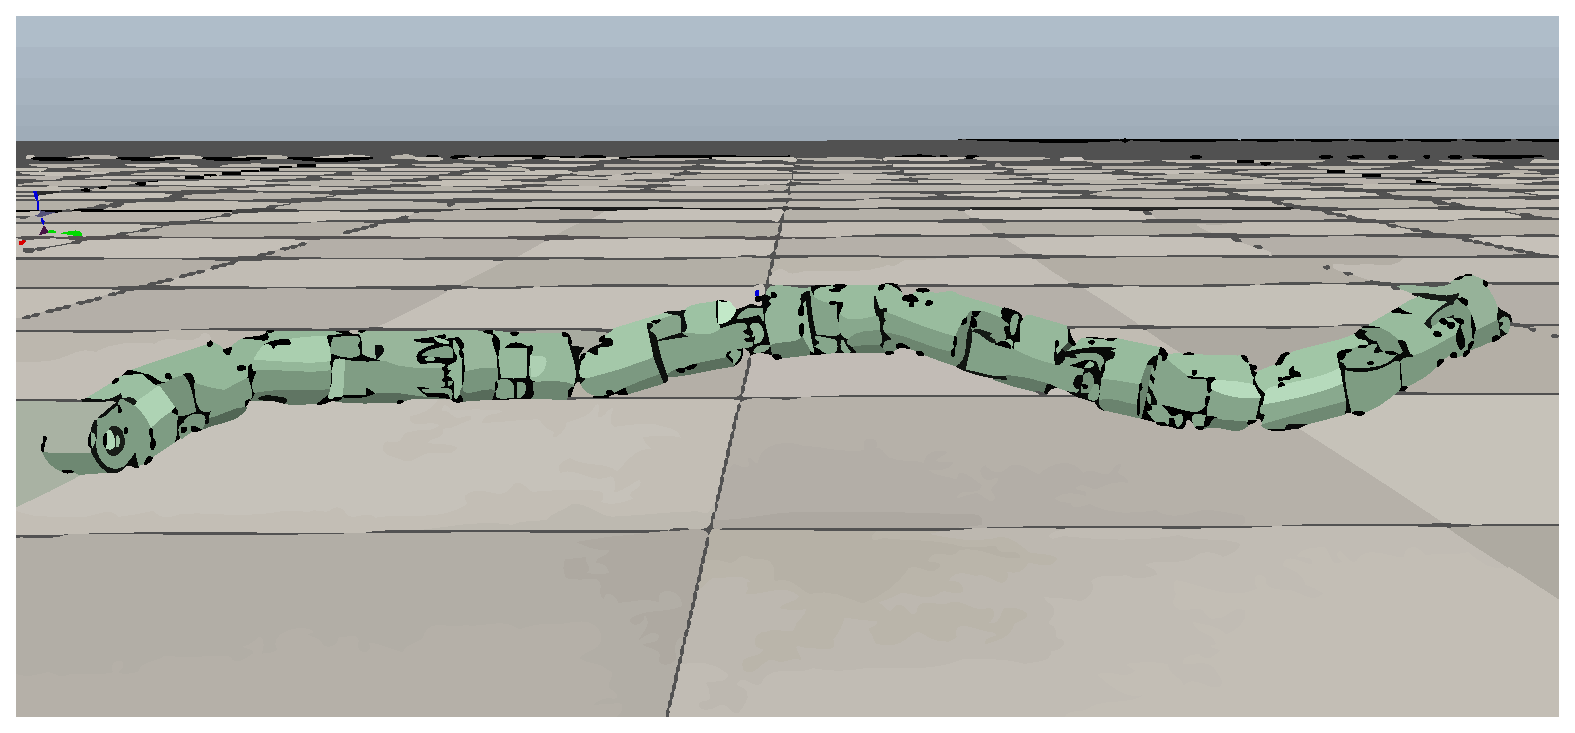
\includegraphics[width=1.5in,height=0.75in]{fig/relative/simulateSnake}
		\figlabel{fig:snake_like_robot_b}
	}
	\caption{The Snake-like robot}
	\figlabel{fig:snake_like_robot}
\end{figure}

The whole process of our control strategy is divided into two parts:

\begin{enumerate}
	\item data acquisition and preprocessing,
	\item real-time data feedback and multi-parameter regression control.
\end{enumerate}

The simulation environment is the pipe climbing, which can be used in cable detection of cable-stayed bridge. In the first part, we collect data in pipes with different diameter as training set. To reduce time of calculation in feed-back control, we adopt clustering algorithm\cite{Cluseter_ICT}\cite{KmeansAndDeepLearning}. In the second part, we apply regression and feed-back control based on previous training data on the motion of robots. We utilize the entropy variance\cite{WaveformEntropyVariance}\cite{EntropyandVarianceasRiskMeasure}\cite{UsingEntropyAndVariance} to measure the effect of the control parameters on the motion and select the most sensitive parameter which has the greatest effect on motion. By transforming the multiple regression into the unit regression and combining the weighted least squares algorithm\cite{gradientMethod}\cite{MSEestimates}, we finally get a fitted regression function and modify the most sensitive parameter.

The contribution of this paper are:

\begin{itemize}
	\item A new framework for robot adaptive control is proposed.
 	This framework greatly reduces the amount of  effort of the regression calculation because of the use of clustering algorithm for data preprocessing as well as the classification of real-time data.
	\item A solution to the problem of multiple regression is proposed.
	Multi-parameter regression is seen as a multiple regression problem. The entropy variance is utilized to select the parameters which are the most sensitive currently, and the rest of the parameters are hysteresis. Therefore, by regressing the sensitive parameter instead of all the parameters, the multiple regression is transformed into the unit regression problem.
\end{itemize}



